\section{Background}

To understand the main idea of this work, this section
acquaints the reader with the necessary
basics. First we go over RDMA:\@ We talk about the current standards
and explain how it achieves better performance than traditional network solutions.

After that, we will cover the basics of fuzzing, which is the main workhorse
of all the types of testing that we exercise. For testing, we make use of a software
version of the RDMA transport, implemented in the Linux Kernel. This section also
covers the fuzzing of the Linux Kernel,
which is different from normal userspace fuzzing.

Lastly, we explain how RDMA applications work
under a popular implementation of the RDMA Verbs library,
namely libibverbs.

\subsection{RDMA}

Remote Direct Memory Access (RDMA) allows one machine to
directly access the memory of a remote machine and increases
performance by using  zero-copy and CPU bypass optimizations\cite{kaliaUsingRDMAEfficiently2014},
which is why this technology has increased in popularity
within data centers and HPC environments in recent years.

These optimizations work as follows. The Direct Memory Access (DMA) engine inside the Network Interface Card (NIC) allows the NIC to
transfer data directly from/to memory without any CPU involvement\cite{pattersonComputerOrganizationDesign2016}.
In this way, a remote computer can request data within the host, and the DMA engine inside
the RDMA-enabled NIC will handle the request. The zero-copy optimization allows the DMA engine to get
the message directly from the user program data space during transmission
and be placed where the user wants it when the message is received,
rather than go through intermediary buffers in the operating system
along the way\cite{pattersonComputerOrganizationDesign2016}.

Initially, RDMA was mostly available within the InfiniBand (IB) architecture,
which defines network protocols over the link, network, and transport layer to move
RDMA packets across the network~\cite{infinibandvol107}. However, The IB network stack requires
specific hardware that is aware of these protocols.

Later came RDMA over Converged Ethernet (RoCE). This specification
made RDMA accessible to the ubiquitous Ethernet technology and is available
in two versions. RoCEv1 replaces the link-layer protocol for the ethernet protocol,
thus enabling the use of regular switches for RDMA services. On top of the modifications
made by RoCEv1, RoCEv2 replaces the network layer protocol of IB for the IP protocol. This
allows routers to transmit RDMA traffic, therefore making RDMA traffic routable under
common hardware. Nevertheless, Communication endpoints still need an RDMA-enabled NIC;\@ for RoCE, this
is called the RoCE adapter card.

SoftRoCE, An open-source software implementation of the RDMA transport, has been part of the mainline tree of
the Linux Kernel since late 2016. SoftRoCE is implemented as a device driver, and it provides a complete RDMA
stack implementation over any regular NIC\cite{softroce}.

Figure~\ref{fig:softroce} shows how SoftRoCE allows a server with commodity hardware (a regular NIC)
and a server equipped with a RoCE adapter card to communicate through RDMA, bridging a gap in the RDMA ecosystem.

\begin{figure}[h!]
  \centering
  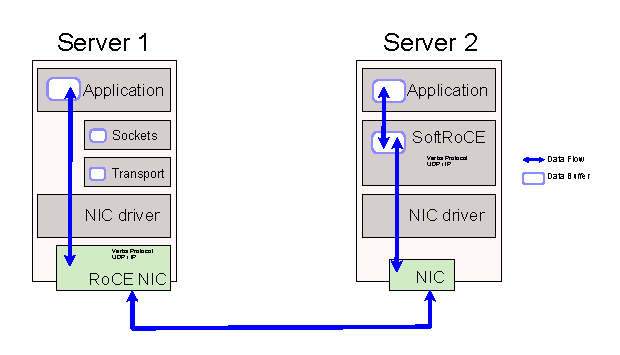
\includegraphics[]{softrocepretty}
  \caption[SoftRoCE]{SoftRoCE allows RDMA interaction with RoCE devices\footnotemark}\label{fig:softroce}
\end{figure}

\footnotetext{adapted from \url{ https://www.roceinitiative.org/wp-content/uploads/2016/11/SoftRoCE_Paper_FINAL.pdf }}

SoftRoCE is very suitable for testing because it does not require any specific
hardware. For this reason, SoftRoCE plays a significant role in this work.

\subsection{The Linux Kernel}

Similar to most Unix kernels, the Linux Kernel is monolithic. All kernel layers
are integrated into a single program, running under the kernel's privileged execution
mode. Because security checks are only enforced by the kernel code,
if there are security vulnerabilities inside the kernel, then the whole system has vulnerabilities\cite{korbethLinuxDeviceDrivers2005}.

One feature of the Linux Kernel is its ability to extend its functionality during runtime using
modules. Modules are pieces of code that can be dynamically linked or unlinked at runtime,
adding functionality to the kernel\cite{korbethLinuxDeviceDrivers2005}. The SoftRoCE driver
and its dependencies for RDMA transport are examples of modules in the Linux Kernel.

\subsection{Fuzzing}

In simple terms, fuzzing is an approach to software testing where a system under test gets bombarded with inputs generated by another program.
The Fuzzer usually monitors the system under test to discover any flaws exposed by the processing of this input\cite{mcnallyFuzzingStateArt2012}.

Generally, these test cases originate from valid inputs after undergoing random modifications. Although modern
fuzzers do not rely solely on randomness for test case generation, the simplicity of this idea yielded great
results. Fuzzing is getting more and more attention in the area of software security and reliability because of its effective
ability to find bugs\cite{liangFuzzingStateArt2018}.

\subsubsection{Fuzzers}

A Fuzzer is a program that generates and delivers inputs for another program. A crucial metric for categorizing Fuzzers is
the amount of knowledge they require over the system under test. Based on this metric, Fuzzers are categorized into 3 main types\cite{mcnallyFuzzingStateArt2012}:

\begin{itemize}
    \item Blackbox Fuzzer: No knowledge of target program internals, the testing process is limited to observing the target's input and output behaviour. Consequently, they have no means of measuring coverage and can only provide input to the target.
    \item Whitebox Fuzzer: These Fuzzers can take advantage of the source code of the target application, not only allowing them better insights into how the system works, but also to benefit from code coverage measurements.
    \item Graybox Fuzzer: This applies to Fuzzers that do not fall into any of the previous categories. Source code of the target may not be available, but other means of inspection such as reverse engineering, static analysis, or executing inside a debugger are the usual workhorses of graybox Fuzzers.
\end{itemize}

With the source code of the target program at hand, a Fuzzer can benefit from coverage information to
better guide the fuzzing process and yield better results. Given a specific input,
the number of basic blocks reached by program execution measures the code coverage.

%% **TODO**

%% Along with coverage, depth is also an important metric when evaluating fuzzing efficiency. A program
%% might reject a test case if, for example, the computed checksum is not equal to the checksum encountered
%% in a fabricated packet. A later step further might reject the input because a header section does not conform
%% to a specific standart. Reaching further stages past  checks inside a program corresponds to reaching greater
%% depths, which is obviously benefitial for succesful fuzzing.

Nowadays, Fuzzers also rely on more advanced techniques like symbolic execution,
taint tracking analysis, and machine learning aided input generation.

\subsubsection{Fuzzer Components}

Fuzzers contain at least some of the following components:

\paragraph{Fuzz Generator:}

A fuzz generator is in charge of creating test inputs to run on the system under test. Different
approaches serve this purpose\cite{mcnallyFuzzingStateArt2012}:

\begin{itemize}\label{ss:fuzzer-components}
    \item Mutative Fuzzer: the idea is to start with a sample input or a set of inputs, and \
    modify a part of it. This set of inputs is commonly refered to as the \textbf{input corpus}; the mutative approach is useful for inputs that must conform to defined structures, coverage is not
    always good. A positive aspect of this type of generators is that they do not require protocol knowledge.
    \item Generative Fuzzer: generates inputs from scratch. This can yield higher coverages, at the cost of requiring
    knowledge of protocols. It can be based on templates or grammars.
\end{itemize}

These two main categories can be further described by the techniques used to generate their data:

\begin{itemize}
    \item Oblivious: generates or mutates data randomly, this brings of course poor coverage.
    \item Template based: provided an input template, the fuzzer will only modify/generate specific parts \
    allowed by the template.
    \item Block based: represent data as nested data blocks of varying types as opposed to string sequences.
    \item Grammar based: make use of a previously given grammar, to generate input.
    \item Protocol fuzzer: knows about concepts such as replies and responses, and in which \
    sequence to reply responses in order to test certain functionality.
\end{itemize}

\paragraph{Coverage guided fuzzing:}

Test case generation based on code coverage is an important aspect for efficient Fuzzers.
The Fuzzer generates a new input based on the input corpus it already has. After
running the target program with this new input, it will collect the code coverage
information and compare it to the previous coverage. If the code coverage is higher after
running the target with this newly generated input, the Fuzzer adds the input to its corpus of inputs.
Algorithm~\ref{alg:genalg} describes this procedure.

\RestyleAlgo{boxruled}
\SetAlgoVlined
\begin{algorithm}[h]
  \caption{Algorithm for Coverage-Based Data Generation}\label{alg:genalg}\LinesNumberedHidden\DontPrintSemicolon
  \KwIn{A set of Inputs $I$}
  \KwOut{An Input Corpus $C$, such that $I \subseteq C$}
  $C \gets I$\;
  $coverageOld \gets 0$\;
  \While{true}{
    $newInput \gets generateInput()$\;
    $coverageNew \gets runTargetProgram(newInput)$\;

    \If{$coverageOld < coverageNew$} {
      $C \gets C \cup \{newInput\} $
    }
    $coverageOld \gets coverageNew$
  }
  \Return{C}
\end{algorithm}

To highlight the importance of using code coverage information to generate new test inputs, consider the program in
Listing~\ref{lst:ifcascade}. Reaching the potential out-of-bounds access would require a blind fuzzer (i.e. without code coverage
information) to go over ${\frac{1}{256}}^{5} = {\frac{1}{2}}^{40}$test cases, in the worst case. %\footnote{${\frac{1}{256}}^{5}$ test cases, as the char type is 8 bits wide.}.

\begin{lstlisting}[caption={If-Cascade Program}, label={lst:ifcascade},  style=CStyle, float, floatplacement=H]
char input[6];

void read_input() {
  fgets(input, 6, stdin);

  if (input[0] == 'o') {
    if (input[1] == 's') {
      if (input[2] == 't') {
        if (input[3] == 'u') {
          if (input[4] == 'd') {
            crash_program();
          }
        }
      }
    }
  }
  operate_normally();
}

void crash_program() {
  int index = random() % 10;
  /* potential out-of-bounds access */
  input[index] = 'S';
}
\end{lstlisting}

If a Fuzzer leverages code coverage information to generate new inputs, the number of input cases it needs to generate
to discover these deeply nested crashes is substantially reduced. In the example of Listing~\ref{lst:ifcascade}, the Fuzzer will consider strings preffixed
with ``o'', ``os'' and ``ost'' to be more interesting, because they trigger new code paths. It will prefer generating strings with these prefixes and
find the crash caused by the out-of-bounds access more efficiently.


\paragraph{Delivery Mechanisms}

A delivery mechanism is a fuzzer component which is in charge of presenting input (from the generator)
to the system under test. Normally, as finding abnormal functioning during regular operation of the
target program is aimed at, Fuzzers use delivery mechanisms simulate those used by the system under test\cite{mcnallyFuzzingStateArt2012}.

Delivery mechanisms are usually one of:

\begin{itemize}
    \item Files,
    \item Environment variables,
    \item Invocation parameters (command-line or Application Programming Interface (API)),
    \item Network transmissions,
    \item Operating system events (including mouse and keyboard events),
    \item Operating system resources,
    \item Direct memory injection (risk to corrupt state and abort program).
\end{itemize}

\paragraph{Monitoring Frameworks}

Detecting that the system under test has crashed as a result of some input is essential to the fuzzing process.
There are two broad classes of monitoring frameworks\cite{mcnallyFuzzingStateArt2012}:

\begin{itemize}
    \item Local monitoring: the fuzzer is installed in the same system as the target. It may look for additional output \
    from the target (such as core dump files) in order to assert that the target has encountered errors.
    \item Remote monitoring: more limited that their counterpart by nature, remote monitowring frameworks recognize \
    a failure by looking for network interruptions.
\end{itemize}
\subsection{Fuzzing the Linux Kernel}\label{ss:fuzzingkernel}

As opposed to userspace fuzzing, fuzzing the Linux Kernel
presents some challenges and limitations. As an example, in single threaded
userspace applications, coverage is a function of the input, it has a
deterministic behaviour; collecting coverage for the kernel however, is
very different;  the kernel contains a high degree
non-deterministic behavior. In~\cite{okechInvestigatingExecutionPath2013}, a
simple test program consisting of an open and a read system call revealed
559 distinct execution paths, which were mainly attributed to interrupts and context switches.

Finding races is another desirable outcome in this scenario. This is
challenging because this kind of bugs depend on exact
execution interleavings of threads to be triggered, they are consequently hardly reproduceable if the testing method does not account for deterministic
thread interleavings.

Despite this challenges, fuzzing has proven to be excelent approach to testing the
kernel's code base: the system call fuzzer Syzkaller alone has discovered
almost  4000 bugs since the time it has been operational as a continous
automated fuzzer\cite{Syzbot}.

The following configuration options are relevant when fuzzing the kernel:

\begin{itemize}
\item The Kernel Address Sanitizer (KASAN): Using compiler instrumentation, validity checks are inserted to memory accesses, thus revealing memory safety errors such as \
  out-of-bound access and use-after-free. For better error reports containing stack traces, one can also enable the option CONFIG\_STACKTRACE along KASAN\cite{KernelAddressSanitizer}.
\item Kcov: kcov exposes coverage information for the kernel in a form suitable for coverage-guided fuzzing. Coverage data is exposed via the kcov debugfs file, located under /sys/kernel/debug/kcov. Kcov \
  aims not to collect as much coverage as possible, but stable coverage (function of the input), by disabling coverage collection from interrupts and from non-deterministic parts of the kernel\cite{KcovCodeCoveragea}
\end{itemize}

%% TODO panic on warn set.

%%
%% despite of this difficulties, talk about limitations of compiler based tools: they cannot discover many errors past more obvious ones.

\subsection{RDMA Applications}

The ``RDMA Verbs Specification' internet draft describes the abstract
interface for RDMA-aware NICs and provides a semantic definition of this
interface. This semantic definition is simply called Verbs\cite{hillandRDMAProtocolVerbs}.

Libibverbs provides an implementation of the Verbs interface\footnote{Hosted at \url{https://github.com/linux-rdma/rdma-core}}. User space
applications can consume the API of libibverbs to interact with
the kernel modules for control path operations and to interact with the drivers asociated
to RDMA-aware devices.

The libibverbs API handles the control path for creation, modification, querying and destruction of resources used by RDMA applications.

For the control path, the library uses system calls that are handled by file operations on device nodes
registered by the uverbs kernel module. The kernel module passes control down to lower-level drivers.
These lower-level drivers can be drivers for real hardware, or drivers for software devices, like SoftRoCE.\@

In contrast to the control path,  the library implements the data path with calls that are made
directly to the low level drivers of the NIC using a doorbell mechanism: the host CPU %via Programmed IO
writes a short doorbell message directly to the
NIC, indicating there is work to be done\cite{kaliaUsingRDMAEfficiently2014}. This data flow mechanism completely circumvents the
host Kernel, enabling the Kernel bypass\cite{kaliaDesignGuidelinesHigh2016}.

The Queue Pair one of the most important resources managed by RDMA applications, it represents an endpoint
in a communication channel. There are different transport modes that can be selected when establishing a Queue Pair\cite{rdmamanual}:

\begin{itemize}
  \item Reliable Connection (RC): A Queue Pair is associated with only one other Queue Pair. Similar to TCP connections, packets are acknowledged and guaranteed to arrive in order.
  \item Unreliable Connection (UC): A Queue Pair is associated with only one other Queue Pair, packet delivery is not guaranteed.
  \item Unreliable Datagram (UD): A Queue Pair may receive or transmit single packets from/to any other UD queue pair.
\end{itemize}

After being created, a Queue Pair is still not ready to receive or send data through a channel; the Queue Pair must be first
transitioned through several states, shown in Figure \ref{fig:qpstatemachine}.

\begin{figure}[h!]
  \centering
  \includegraphics[height=8cm, keepaspectratio]{qpstatemachine}
  \caption[Queue Pair state machine]{The Queue Pair state machine, slightly adapted from~\cite{QPStateMachine2012}.}
  \label{fig:qpstatemachine}
\end{figure}

The Queue Pair consists of two Work Queues, a Send Queue and a Receive
Queue. The Work Queues handle sending and receiving messages.
An application can post Work Requests in the context of a Queue Pair, in
doing so, the application asks the RDMA device to handle the task.
A Work Request can be polled for completion, this operation will yield
the status of the Work Request that was posted. Depending on the transport
mode and the Work Request, a successful status can depend on the receiver
side to answer with an acknowledgment packet.

Directly after creation, a Queue Pair is in a Reset state. In the Reset state,
a Queue Pair cannot post any Work Requests to any
of its Work Queues, and any packets it receives will be silently dropped.
A Queue Pair can transition from one state to another when the program calls ibv\_modify\_qp() ---
transitions marked with blue in Figure~\ref{fig:qpstatemachine} originate from this function call.
Work Requests may be posted to the Receive Queue once the Queue Pair has transitioned to a Ready To Receive (RTR) state,
similarly Work Requests may be posted to the Send Queue after reaching the Ready To Send (RTS) state. The Queue Pair will silently drop
packets until it has at least reached the RTR state.

The Send Queue Error (SQE) state transition happens automatically
after a Work Request in the Send Queue ends with an error\cite{QPStateMachine2012}. The Send Queue Drain (SQD) is a special state
that won't process further Work Requests posted to the Send Queue\cite{QPStateMachine2012}. Both the SQD and SQE state handle incoming packets\cite{barakVerbsProgrammingTutorial2014}.

Errors ocurring during the ibv\_modify\_qp() call will bring the Queue Pair
to the Error state, Work Request errors may transition the Queue Pair to this state as well\cite{QPStateMachine2012}.

\subsubsection{Transport Layer: The Base Transport Header}

One of the tasks of low level drivers for RDMA devices is to process
packet headers of the transport layer protocol. This task roughly consists
of assigning a queue pair to the packet, performing requested memory access operations like
read or write and performing sanity checks.

These transport layer headers are called
base transport headers, and contain information describing the
requested operation and the  destination queue pair.

There are also header extensions for the base header, but their presence is dictated
by the operation code. We will focus in this section on base transport header,
because they are common to all RDMA traffic.

Base transport headers are 96 bits long, Table~\ref{tab:bthfields} shows the corresponding field descriptions. The order in which fields
are listed in Table~\ref{tab:bthfields} coincide with the layout of the actual header.

\begin{table}[h]
  \begin{tabular}{| m{10em} | m{3em} | m{15em} |}
    \hline
    Field Name &  Field Size (bits) & Description\\
    \hline
    Opcode & 8 & Indicates the packet type, also specifies which extension headers follow the base transport header.\\
    \hline
    Solicited Event & 1 &  The requester sets this bit to 1 to specify that the responder shall invoke the Completion Queue event handler.\\
    \hline
    MigReq & 1 &  Used to communicate Path Migration State, path migration refers to both communication partners agreeing to use a new communication path\\
    \hline
    Pad Count & 2 &  Number of pad bytes added to the headers to align the payload to a 4 byte boundary.\\
    \hline
    Transport Header Version & 4 &  Specifies the Transport version used for the packet, it is set to 0x0.\\
    \hline
    Partition Key & 16 &  Partitioning allows isolation among systems sharing the same fabrics. If using partition, this field is required to match partition key stored at the receiver or else the packet will be discarded\\
    \hline
    Reserved & 8 &  transmited as 0s, this field is ignored on the receiver side.\\
    \hline
    Destination QP & 24 &  specifies a number to identify the destination queue pair.\\
    \hline
    Acknowledge Request & 1 &  If this bit is set, responder should schedule an acknowledgment packet on the associated queue pair.\\
    \hline
    Reserved & 7 &  transmited as 0s, ignored by receiver. \\
    \hline
    Packet Sequence Number & 24 &  Identifies the position of a packet in a sequence of packets, used e.g. to recognize lost packets.\\
    \hline
  \end{tabular}
  \caption[Base Transport Header Fields]{Base Transport Header Fields, adapted from\cite{infinibandvol107}}
  \label{tab:bthfields}
\end{table}

\subsubsection{Challenges posed for Fuzzing}\label{s:ibverbs-challenges}

Reaching full coverage for RDMA Verbs applications is not trivial. In order to perform RDMA operations, establishment of
a connection to the remote host, as well as appropriate permissions need to be set up first. The mechanism for accomplishing
these tasks is the Queue Pair\cite{rdmamanual}. A Queue Pair defined for connected transport modes needs information from
the remote Queue Pair in order to transition to a ready state.

At the time the device driver checks the Base Transport Headers, it will also assert if there is an existing Queue Pair
with the Queue Pair number found in the Destination QP field in the header.
It will also check if this queue pair is in a ready state; if any of these conditions
are not met, the driver will drop the packet.

This means that a fuzzing application should either let 2 applications initialize and reach a ready state,
or lead the target application to think it has connected with another application. As we have seen
in the previous sections, Queue Pairs are modeled by a state machine and they must be carefully transitioned from one
state to another. Since driver code enforces that the Queue Pair must be in a specific state for operations like
handling incoming packets, there might be bugs that are tied to specific states. It is meaningful to test
RDMA applications running in a connected environmnent.
